\documentclass[paper=letter]{scrartcl}

\usepackage[T1]{fontenc}
\usepackage{color}
% if you don't have this font, please 
% get it from http://www.ctan.org/tex-archive/fonts/libertine/
% or simply comment out the line below
%\usepackage{libertine}
\usepackage{bookman}


\usepackage{listings}
\usepackage{graphicx}
\usepackage{fancyvrb}
\usepackage{hyperref}

\newcommand{\cppFile}[1]{\texttt{#1}}
\newcommand{\inputItem}[1]{\noindent\texttt{\bf #1} ---}
\newcommand{\inputSubItem}[1]{\indent\texttt{\it #1} --}
%% Remove the below command before submission
\newcommand{\todo}[1]{\textcolor{red}{#1}}
%Format to denote a C++ class name:
\newcommand{\cppClass}[1]{{\sffamily #1}}
%Format to denote a C++ variable: 
\newcommand{\cppFunction}[1]{{\tt #1}}
% for the cover page:
\newcommand{\HRule}{\noindent\rule{\linewidth}{1.5pt}}
\hyphenation{Wave-Function-Transformation}
\lstset{language=c++,basicstyle=\footnotesize\ttfamily,keywordstyle=\color{blue}\bfseries,frame=shadowbox}
\begin{document}

\begin{titlepage}
\vspace*{\stretch{1}}
\HRule
\begin{flushright}
\LARGE  DMRG++ v2.0 Manual
\end{flushright}
\HRule
\vspace*{\stretch{2}}



%
\begin{center}
\textsc{Oak Ridge, 2009}
\end{center}

\end{titlepage}
% 
\begin{titlepage}
\noindent
\begin{minipage}{0.4\textwidth}
\begin{flushleft}
Gonzalo \textsc{Alvarez}\\
Nanomaterials Theory Institute\\
Oak Ridge National Laboratory\\[0.2cm]
Oak Ridge, TN 37831\\
\today
\end{flushleft}
\end{minipage}

\vspace*{\stretch{2}}
\noindent
%\begin{minipage}{0.6\textwidth}
\begin{tiny}
\fontshape{sc}\selectfont
%\begin{verbatim}
\noindent
DISCLAIMER\\[0.2cm]
THE SOFTWARE IS SUPPLIED BY THE COPYRIGHT HOLDERS AND
CONTRIBUTORS "AS IS" AND ANY EXPRESS OR IMPLIED
WARRANTIES, INCLUDING, BUT NOT LIMITED TO, THE IMPLIED
WARRANTIES OF MERCHANTABILITY AND FITNESS FOR A
PARTICULAR PURPOSE ARE DISCLAIMED. IN NO EVENT SHALL THE
COPYRIGHT OWNER, CONTRIBUTORS, UNITED STATES GOVERNMENT,
OR THE UNITED STATES DEPARTMENT OF ENERGY BE LIABLE FOR
ANY DIRECT, INDIRECT, INCIDENTAL, SPECIAL, EXEMPLARY, OR
CONSEQUENTIAL DAMAGES (INCLUDING, BUT NOT LIMITED TO,
PROCUREMENT OF SUBSTITUTE GOODS OR SERVICES; LOSS OF USE,
DATA, OR PROFITS; OR BUSINESS INTERRUPTION) HOWEVER
CAUSED AND ON ANY THEORY OF LIABILITY, WHETHER IN
CONTRACT, STRICT LIABILITY, OR TORT (INCLUDING NEGLIGENCE
OR OTHERWISE) ARISING IN ANY WAY OUT OF THE USE OF THIS
SOFTWARE, EVEN IF ADVISED OF THE POSSIBILITY OF SUCH
DAMAGE.

NEITHER THE UNITED STATES GOVERNMENT, NOR THE UNITED STATES DEPARTMENT OF ENERGY, 
NOR THE COPYRIGHT OWNER, NOR
ANY OF THEIR EMPLOYEES, REPRESENTS THAT THE USE OF ANY
INFORMATION, DATA, APPARATUS, PRODUCT, OR PROCESS
DISCLOSED WOULD NOT INFRINGE PRIVATELY OWNED RIGHTS.\\[1cm]

\fontshape{\shapedefault}\selectfont
%\end{verbatim}
\end{tiny}
%\end{minipage}
\noindent
\begin{minipage}{0.4\textwidth}
Copyright \copyright 2009, UT-Battelle, LLC\\
All rights reserved
\end{minipage}
\hfill
\begin{minipage}{0.4\textwidth}
\begin{flushright}

\includegraphics[width=3cm]{dmrgV2LogoBW.png}
\end{flushright}
\end{minipage}
\end{titlepage}
\tableofcontents

\begin{center}

\includegraphics[width=2cm]{Under_construction_icon-blue}\\
{\tiny http://commons.wikimedia.org/wiki/File:Under\_construction\_icon-blue.svg}
\end{center}
\pagebreak

\section{Introduction}
%METAExtractStartREADME
\subsection{Licensing}
The full software license for DMRG++ version 2.0.0 
can be found in
%METaIgnoreNextLine
appendix \todo{FIXME}, and in
file LICENSE in the root directory of the code.
DMRG++ is a free and open source implementation of the 
DMRG algorithm. You are welcome to use it and publish data 
obtained with DMRG++. If you do, please cite this
work (see next subsection).

\subsection{How To Cite This Work}\label{subsec:citeme}
\begin{Verbatim}
@article{re:alvarez09,
author="G. Alvarez",
title="The density matrix renormalization group for strongly correlated electron
systems: A generic implementation",
journal="Computer Physics Communications",
volume="180",
pages="1572",
year="2009"}
\end{Verbatim}
And also:
\begin{Verbatim}
@article{
re:webDmrgPlusPlus,
Author = {G. Alvarez},
Title = {DMRG++ Website},
Publisher = {\url{http://www.ornl.gov/~gz1/dmrgPlusPlus}} }
\end{Verbatim}

%METAExtractStartCHANGES
\subsection{What's new in Version 2}
\begin{itemize}
\item Engine: SU(2) symmetry now supported and integrated
\item Engine: Checkpointing
\item Engine: DiskStack to support checkpointing
\item Engine: Faster\footnote{Faster but not fast.} WaveFunctionTransformation for local symmetries
\item User Interface: Customizable finite sweeps
\item New Model: FeBasedSc for Fe-based Superconductors
\item New Geometry: GeometryLadderFeAs to go with FeBasedSc
\item Tests: TestSuite added (under /TestSuite)
\item Documentation: Manual added (under /doc)
\end{itemize}
%METAExtractEndCHANGES

\section{Building and Running DMRG++}
\subsection{Required Software}
\begin{enumerate}
\item (required) GNU C++
\item (required) The LAPACK library.
This library is available for most platforms.
The configure.pl script will ask for the LDFLAGS variable 
to pass to the compiler/linker. If the linux platform was
chosen the default/suggested LDFLAGS will include -llapack.
If the osx platform was chosen the default/suggested LDFLAGS will
include  -framework Accelerate.
For other platforms the appropriate linker flags must be given.
More information on LAPACK is here: http://netlib.org/lapack/
\item (optional) make or gmake (only needed to use the Makefile)
\item (optional) perl (only needed to run the configure.pl script)
\end{enumerate}

\subsection{Quick Start}
To Build DMRG++:
\begin{verbatim}
cd src
perl configure.pl
(please answer questions regarding model, etc)
make
\end{verbatim}

To Run DMRG++:
\begin{verbatim}
./dmrg input.inp
\end{verbatim}

The files created by \cppFile{configure.pl} are the following:

\cppFile{main.cpp}: 
\cppFile{configure.pl} will create the file \cppFile{main.cpp}
which contains the entry point (function int main()) for DMRG++,
according to the answers to questions given.

\cppFile{Makefile}:
\cppFile{configure.pl} will create the file \cppFile{Makefile}
according to the answers to questions given. 
In the Makefile, LDFLAGS must contain the linker flags to 
link with the LAPACK library. Defaults provided 
 automatically by configure.pl should work in most cases.
If MPI is not selected (serial code) then the compiler will be chosen to be g++.
Other compilers may work but only the GNU C++ compiler, g++, was tested.
If MPI is selected then the compiler will be chosen to be mpicxx, which 
is usually a wrapper script around g++ to take care of linking with MPI libraries 
and to include MPI headers. Depending on your MPI installation you might need to
change the name of this script.

\cppFile{input.inp}:
\cppFile{configure.pl} will create the file \cppFile{input.inp}
according to the answers to questions given.
This file can be used as input to run the DMRG++ program, in the following way:
for serial code:
\begin{verbatim}
./dmrg input.inp
\end{verbatim}
for MPI code: (actual command will vary according to MPI Installation):
\begin{verbatim}
mpirun ./dmrg input.inp
\end{verbatim}
%METADisableREADME

\section{User's Guide}
%METAEnableREADME
\subsection{Input File}
There is a single input file that is passed as the first
and only argument to the program.
There are two kinds of parameters in the input file:
(i) model parameters, and (ii) DMRG Solver parameters.
The Model parameters vary from model to model.
The DMRG Solver parameters are discussed below.

\inputItem{Options}
A comma-separated list of strings. At least one of the following strings must be provided:
\inputSubItem{none}  Use this when no options are given, since the list of strings must be non-null.
Note that ``none'' does not disable other options.\\
\inputSubItem{hasQuantumNumbers} If this option is given, the program will read the line ``QNS'' 
described below and act accordingly. It is recommended that you set this option.  \\
\inputSubItem{wft}  Use the Wave Function Transformation speed-up, which is disabled by default.\\
\inputSubItem{useSu2Symmetry} Use the SU(2) symmetry for the model, and interpret quantum numbers in 
the line ``QNS'' appropriately. The option ``hasQuantumNumbers'' must be set for this to work.\\
\inputSubItem{nofiniteloops}  Don't do finite loops, even if provided under ``FiniteLoops'' below.\\
%
\inputItem{version}  A mandatory string that is read and ignored. Usually contains the result
of doing ``git rev-parse HEAD''.\\
\inputItem{outputfile}  The output file. This file will be created if non-existent, and if it
exits it will be truncated.\\
\inputItem{InfiniteLoopKeptStates}  ``m'' value for the infinite algorithm.\\
\inputItem{FiniteLoops} A series of space-separated numbers. More than one space is allowed.
The first number is the number of finite algorithm ``movements'', followed by series
of three numbers for each ``movement''. Of the three numbers, the first
is the number of sites to go forward if positive or backward if negative.
The second number is the ``m'' for this ``movement' and the last number is either 0 or 1,
0 will not save state data to disk and 1 will save all data to be able to calculate observables.
The first ``movement'' starts from where the infinite loop left off, at the middle of the lattice.\\
\inputItem{QNS}  A space-separated list of numbers. More than one space is allowed.
The first number is the number of numbers to follow, these numbers being the density of quantum
numbers for each conserved quantum number to be used.
In a simpler way, usually this is 3 followed by $n_\uparrow n_\downarrow 0$  if not using
SU(2) symmetry, where  $n_\uparrow$, and $n_\downarrow$ are the densities of up and down
electrons respectively. If there is SU(2) symmetry then this is 3 followed by $n_\uparrow n_\downarrow j$,
where $n_\uparrow$, and $n_\downarrow$ are the densities of up and down
electrons respectively, and $j$ is twice the angular momentum divided by the number of sites.
%METAExtractEndREADME

\subsection{Finite Loops}

\subsubsection{Enabling finite loops}
There are two ways:
\begin{enumerate}
\item When you run configure.pl you can add as many finite loops as you want.
\item After running configure.pl you can tailor the input.inp file produced by
configure.pl as you want. Note that if you run configure.pl again input.inp will
be overwritten. Make a backup copy.
\item Make sure the input file does \emph{not} have the option \verb=nofiniteloops=
\end{enumerate}

\subsubsection{Finite loop related items in the input file}
\begin{itemize}
\item
{\bf options line:} \verb=nofiniteloops=: Don'��t do finite loops, even if provided under {\bf FiniteLoops} below.
\item {\bf InfiniteLoopKeptStates} $m$�� value for the infinite algorithm.
\item {\bf FiniteLoops} A series of space-separated numbers. More than one space is allowed. The first
number is the number of finite algorithm ``movements''��, followed by series of three numbers for
each ``movement''. Of the three numbers, the first is the number of sites to go forward if positive
or backward if negative. The second number is the $m$ for this movement and the last number
is either 0 or 1, 0 will not save state data to disk and 1 will save all data to be able to calculate
observables. The first movement starts from where the infinite loop left off, at the middle of the
lattice.
\end{itemize}

\subsubsection{Example of a Finite loops line in the input file}
\begin{verbatim}
FiniteLoops 4 7 200 0 -7 200 0 7 200 1 7 200 1
\end{verbatim}
The number 4 implies 4 finite loops. The first fine loop is ``7 200 0'', meaning
go forward 7 steps, use $m=200$ for this finite sweep, and 0: do not store transformation in disk.
The next is ``-7 200 0'', which goes backwards 7 sites, etc.
Remember that the finite loops start at the middle of the lattice, where the infinite loop left off.
ADD FIGURE SHOWING WHAT THIS DOES.

\subsubsection{Caveats and Troubleshooting}
\begin{itemize}
\item If \verb=nofiniteloops= is an option in the options line of the input file then
the {\bf FiniteLoops} line in the input file is ignored, and no finite loops are done. 
In this case, DMRG++ stops when the infinite algorithm has finished.

\item The syntax of the {\bf Finiteoops} line is not checked against errors. 
\item Make sure the first number is the number of triplets that follow. 
\item Make sure
you don't fell off the lattice, by going forward or backwards too much.
Remember that at least one site must remain for the ``system'' part of the lattice.
So on a 16 site chain, when you start the finite loops you're at the middle, you
can go forward at most 7 sites, and backwards at most 7 sites.
\item Future work will provide user-friendly errors when these mistakes are made.
For now \emph{caveat user!}
\end{itemize}

\section{Main Driver}
The high level program is this
\begin{lstlisting}
//! Setup the Model
ModelType model(mp,dmrgGeometry);

//! Setup the dmrg solver:
SolverType dmrgSolver(dmrgSolverParams,model,concurrency);

//! Perform DMRG Loops:
dmrgSolver.main();
\end{lstlisting}


\todo{Graphic showing the template dependencies of the classes}

\section{DMRG Engine}
\subsection{DMRG Algorithm}
Let us define {\it block} to mean a finite set of sites. 
Let $C$ denote the states of a single site. This set is model dependent. For the Hubbard model it is given by:
$C=\{e,\uparrow,\downarrow,(\uparrow,\downarrow)\}$, where $e$ is a formal element that denotes an empty state.
For the t-J model it is given by  $C=\{e,\uparrow,\downarrow\}$, and for the Heisenberg model by  $C=\{\uparrow,\downarrow\}$. 
A {\it real-space-based Hilbert space} $\mathcal{V}$ on a block $B$ and  set $C$ is a 
 Hilbert space with basis $B^{C}$.  I will simply denote this as $\mathcal{V}(B)$ and assume that $C$ 
 is implicit and fixed.
A {\it real-space-based Hilbert space} can also be thought of as the external product space of $\#B$ Hilbert spaces on a site, one for each
 site in block $B$.
We will consider general Hamiltonians   that
 act on Hilbert spaces $\mathcal{V}$, as previously defined.

I shall give a procedural description of the DMRG method in the following.
We start with an initial block $S$ (the initial system) and $E$ (the initial environment). 
Consider two sets of blocks $X$ and $Y$. 
We will be adding blocks from $X$ to $S$, one at a time, and from $Y$ to $E$, one at a time. 
Again, note that $X$ and $Y$ are sets of blocks whereas $S$ and $E$ are blocks. This is shown schematically in Fig.~\ref{fig:sxye}.
All sites in $S$, $X$, $Y$ and $E$ are numbered as shown in the figure.
\begin{figure}
\centering{
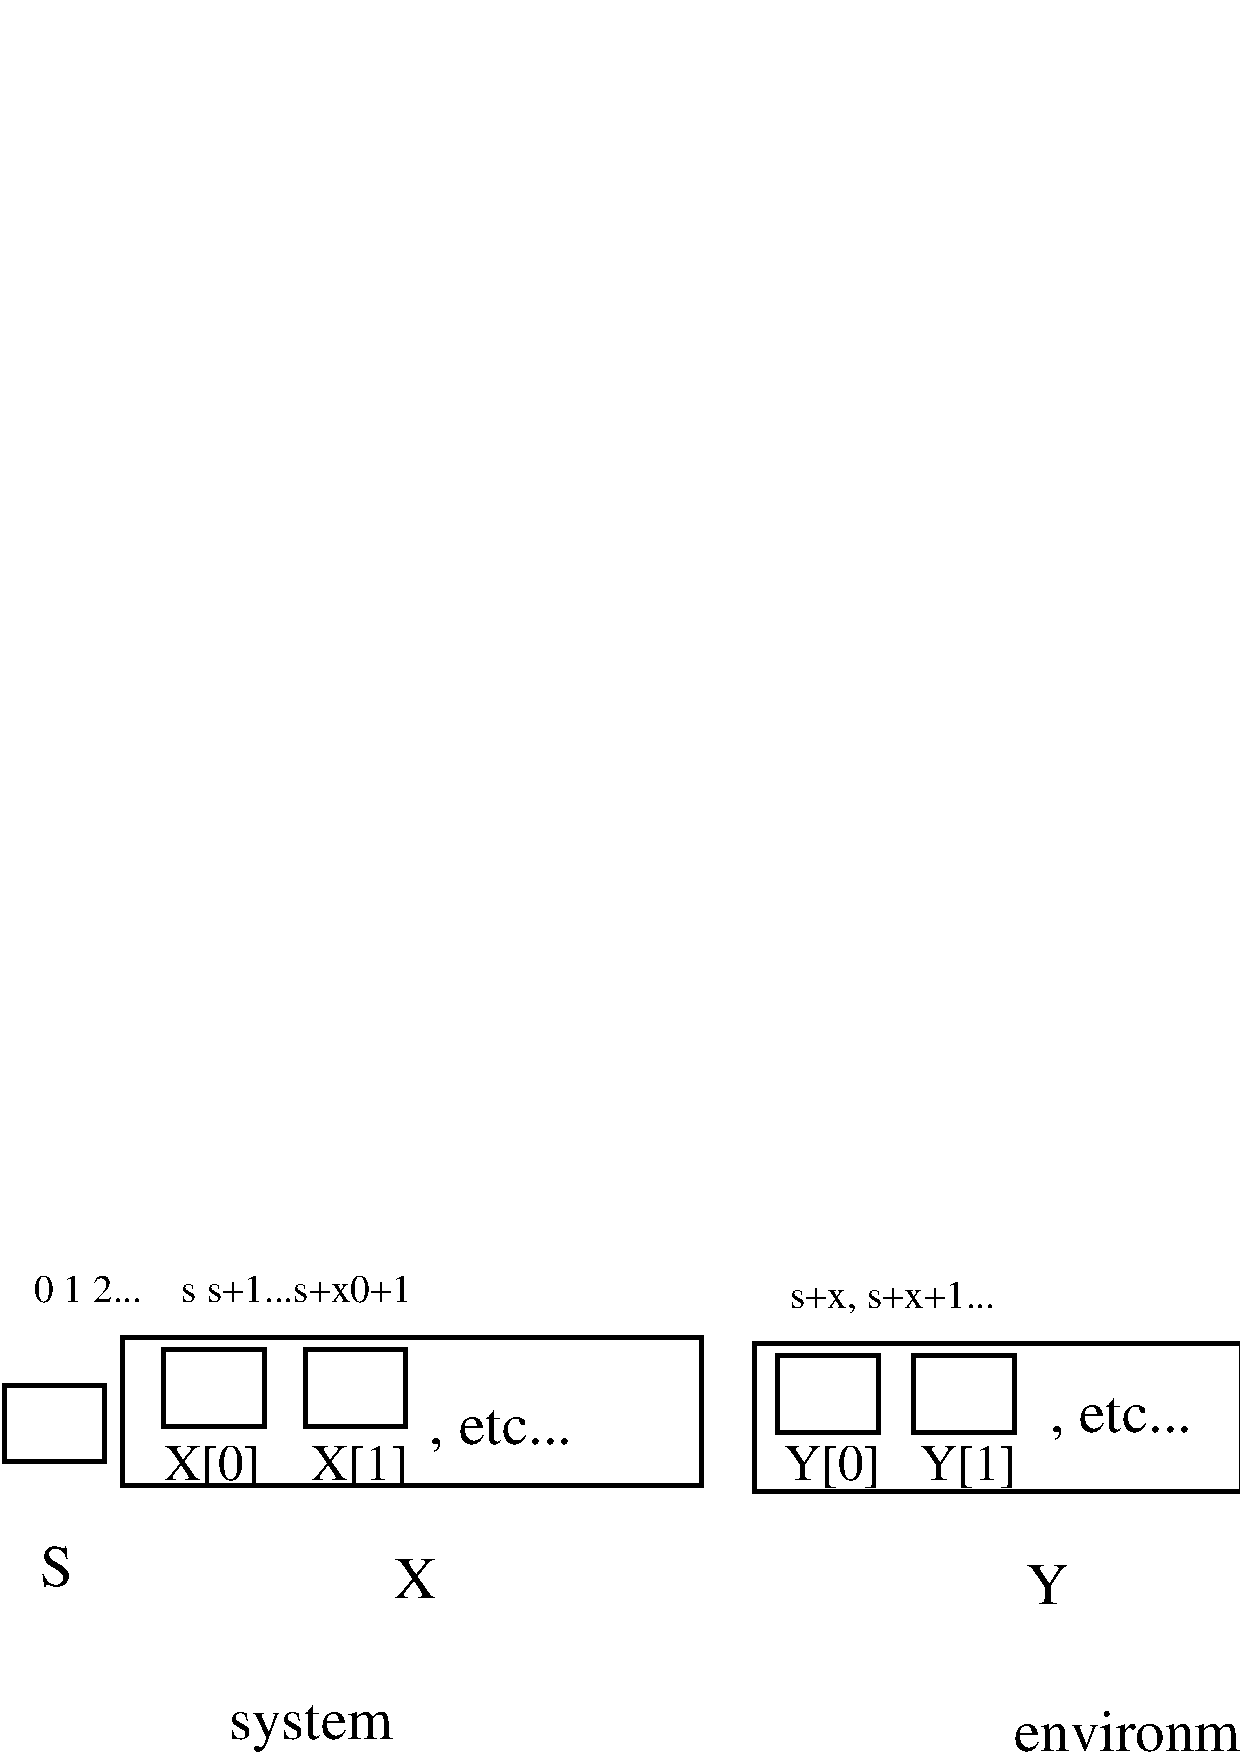
\includegraphics[width=8cm]{dmrg_sxye}}
\caption{Labeling of blocks for the DMRG procedure. Blocks from  vector of blocks X are added one at a time to block $S$ to form 
the system and blocks from  vector of blocks
Y are added one at a time to E to form the environment. Blocks are vectors of integers. The integers (numbers at the top of the figure)
label all sites in a fixed and unique way.\label{fig:sxye}}
\end{figure}
Now we start a loop for the DMRG ``infinite'' algorithm
 by setting $step=0$ and $\mathcal{V}_R(S)\equiv\mathcal{V}(S)$ and $\mathcal{V}_R(E)\equiv\mathcal{V}(E)$.

The system is grown by adding the sites in $X_{step}$ to it, and let
 $S'=S\cup X_{step}$, i.e. the $step$-th block of $X$ to $S$ is added to form the block $S'$; likewise, let $E'=E\cup Y_{step}$. 
Let us form the following product Hilbert spaces:
$\mathcal{V}(S')=\mathcal{V}_R(S)\otimes \mathcal{V}(X_{step})$ and 
$\mathcal{V}(E')=\mathcal{V}_R(E)\otimes \mathcal{V}(Y_{step})$ and their union $\mathcal{V}(S')\otimes\mathcal{V}(E')$ which is disjoint.

Consider $\hat{H}_{S'\cup E'}$, the Hamiltonian operator, acting on $\mathcal{V}(S')\otimes\mathcal{V}(E')$.
Using Lanczos\ref{sec:lanczos},
we  diagonalize $\hat{H}_{S'\cup E'}$ to obtain its lowest eigenvector:
\begin{equation}
|\psi\rangle = \sum_{\alpha\in \mathcal{V}(S'), \beta\in\mathcal{V}(E')}\psi_{\alpha,\beta}|\alpha\rangle\otimes|\beta\rangle,
\label{eq:psi}
\end{equation}
where $\{|\alpha\rangle\}$ is a basis of $\mathcal{V}(S')$ and $\{|\beta\rangle\}$ is a basis of $\mathcal{V}(E')$.

Let us define the density matrices for system:
\begin{equation}
(\hat{\rho}_S)_{\alpha,\alpha'} = \sum_{\beta\in\mathcal{V}(E')}\psi_{\alpha',\beta}^*\psi_{\alpha,\beta}
\label{eq:rhoSystem}
\end{equation}
in $\mathcal{V}(S')$,
and environment:
\begin{equation}
(\hat{\rho}_E )_{\beta,\beta'}= \sum_{\alpha\in \mathcal{V}(S')}\psi_{\alpha,\beta'}^*\psi_{\alpha,\beta}
\label{eq:rhoEnviron}
\end{equation}
in $\mathcal{V}(E')$.
We then diagonalize $\hat{\rho}_S$, and obtain its eigenvalues and eigenvectors, 
$w^S_{\alpha,\alpha'}$ in $\mathcal{V}(S')$ ordered in decreasing eigenvalue order.
We change basis for the operator $H^{S'}$ (and other operators as necessary), as follows:
\begin{equation}
(H^{S' {\rm new\,\,basis}})_{\alpha,\alpha'}=(w^S)^{-1}_{\alpha,\gamma} (H^{ S'})_{\gamma,\gamma'}w^S_{\gamma',\alpha'}.
\label{eq:transformation}
\end{equation}
We proceed in the same way for the environment,  diagonalize $\hat{\rho}_E$ to obtain ordered
eigenvectors $w^E$, and define $(H^{ E' {\rm new\,\,basis}})_{\alpha,\alpha'}$.

Let $m_S$ be a fixed number that corresponds to the number of states in $\mathcal{V}(S')$ that we want to keep. 
Consider the first $m_S$ eigenvectors $w^S$, 
 and let us call the Hilbert space spanned by them, $\mathcal{V}_R(S')$, the DMRG-reduced Hilbert space on 
block $S'$. If $m_S\ge\#\mathcal{V}(S')$ then we keep all eigenvectors and there is effectively no truncation.
We truncate the matrices $(H^{S' {\rm new\,\,basis}})$ (and other operators as necessary)
such that they now act on this truncated Hilbert space, $\mathcal{V}_R(S')$.
We proceed in the same manner for the environment.%

Now we increase $step$ by 1, set $S\leftarrow S'$, $\mathcal{V}_R(S)\leftarrow\mathcal{V}_R(S')$, 
 $H_{S'}\leftarrow H_{S}$,
 and similarly for the environment, and continue with the growth phase of the algorithm.

In the infinite algorithm, the  number of sites in the
 system and environment grows as more steps are performed.
After this infinite algorithm, a finite algorithm is applied where the environment is shrunk at the expense of the system, and the system is grown
at the expense of the environment. During the finite algorithm (\todo{Section to be written}) phase the total number of sites remains constant allowing for a formulation
of DMRG as a variational method in a basis of matrix product states.
The advantage of the DMRG algorithm is that the truncation procedure described above keeps the error bounded and small.
Assume $m_S=m_E=m$.
At each DMRG step\cite{re:dechiara08} the truncation error $\epsilon_{tr}=\sum_{i>m} \lambda_i$, where $\lambda_i$ are the eigenvalues of the
truncated density matrix $\rho_S$ in decreasing order. The parameter $m$ should be chosen such that $\epsilon_{tr}$ remains small, say \cite{re:dechiara08}
$\epsilon_{tr}<10^{-6}$. For critical 1D systems $\epsilon_{tr}$ decays as a function of $m$ with a  power law, while for 1D system
away from criticality it decays exponentially. For a more detailed description of the error introduced by the DMRG truncation in other
systems see \cite{re:dechiara08,re:schollwock05,re:hallberg06,re:rodriguez02}.

\subsection{Driver Program}
Let us motivate the discussion by introducing a typical problem to be solved by DMRG: ``Using the DMRG method, 
one would like to calculate the local density of states on all sites for a Hubbard model with
inhomogeneous Hubbard U values on a one-dimensional (1D) chain''.
We want to modularize as many tasks mentioned in the last sentence as possible. We certainly want to separate the DMRG solver from the model in question,
since we could later want to do the same calculation for the t-J model; and
the model from the lattice, since we might want to do the same calculation on, say, a n-leg ladder, instead of a 1D chain.
C++ is a computer language that is very fit for this purpose, since it allows to template classes. 
Then we can write a C++ class to implement the DMRG method (\cppClass{DmrgSolver} class),  and template this class 
on a strongly-correlated-electron (SCE) model template, so that we can delegate all SCE model related code to the SCE model class.

However, for DmrgSolver to be able to use a given SCE model, we need a convention that such SCE model class
will have to follow.
This is known as a C++ public interface, and for a SCE model it is given in  \cppClass{DmrgModelBase}. 
To do the calculation for a new SCE model, we simply need to
 implement all functions found in \cppClass{DmrgModelBase}  \emph{without} changing the \cppClass{DmrgSolver} class. 
The model will, in turn, be templated on the geometry. For example, the Hubbard model  with
inhomogeneous Hubbard U values and inhomogeneous hoppings (class \cppClass{DmrgModelHubbard}) 
delegates all geometry related operations to a templated geometry class.
Then \cppClass{DmrgModelHubbard} can be used for, say, one-dimensional chains and n-leg ladders \emph{without} modification.
This is done by just instantiating
 \cppClass{DmrgModelHubbard} with the appropriate
geometry class, either \cppClass{DmrgGeometryOneD} or 
\cppClass{DmrgGeometryLadder}, or some other class that the reader may wish to write, which implements the interface given in
\cppClass{DmrgGeometryBase}. 
\todo{Add figure showing interfaces}

In the following sections I will describe these different modules. Since the reader
may wish to first understand how the DMRG method is implemented, I will start with the core C++ classes that implement the method.
The user of the program
will not need to change these core classes to add functionality. Instead, new models and geometries can be added by creating implementations
for \cppClass{DmrgModelBase} and \cppClass{DmrgGeometryBase}, and those public interfaces will be explained next.

But for now I end this section by briefly describing the ``driver'' program  for a Hubbard model on a 1D chain (see file main.cpp).
There, \cppClass{DmrgSolver} is instantiated with \cppClass{DmrgModelHubbard}, since in this case one wishes to perform the calculation for the Hubbard model.
In turn, \cppClass{DmrgModelHubbard}  is instantiated with  \cppClass{DmrgGeometryOneD} since now one wishes to perform the calculation on a 1D chain.

\todo{Expand the driver explanation}

\subsection{DmrgSolver and The ``Infinite'' DMRG Algorithm}
The purpose of the \cppClass{DmrgSolver} class is to perform  the loop for the DMRG ``infinite algorithm'' discussed before.
This class  also performs  
the ``finite algorithm''  \cite{re:schollwock05} to allow for the calculation of static (and in the future dynamic) 
observables, such as static correlations.

The program is structured as a series of header files containing the 
implementation\footnote{Traditionally, implementation is written in cpp files that are compiled separately. However, here templates
are used heavily, and to avoid complications related to templates that some C++ compilers cannot handle,
 we choose to have only one translation unit.} with each class written in the header file of the same name, 
 and a ``driver'' program that uses the
capabilities provided by the header files to solve a specific problem.
To simplify the discussion, we start where the ``driver program'' starts, in its \cppFunction{int main()} function, 
which calls \cppFunction{dmrgSolver.main()}, whose main work is to perform  the loop for the 
``infinite'' DMRG algorithm. Let us now discuss this loop which is found in the \cppFunction{infiniteDmrgLoop} function, 
and is sketched in Fig.~\ref{fig:infiniteloop}.

\begin{figure}
\begin{lstlisting}
for (step=0;step<X.size();step++) {
  // grow system (a)		
  grow(pSprime,pS,X[step],model,GROW_RIGHT);
  // grow environment (b)
  grow(pEprime,pE,Y[step],model,GROW_LEFT; 
  // product of system and environment (c)   
  pSE.setToProduct(pSprime,pEprime); 				
  
  diagonalize(psi,pSprime,pEprime,pSE,
       model); // (d)			
  ns=pSprime.size();
  ne=pEprime.size();
  changeAndTruncateBasis(pS,psi,pSprime,ns,ne,
    pSE,0); // (e)
  changeAndTruncateBasis(pE,psi,pEprime,ns,ne,
    pSE,1); // (f)
    
  systemStack.push(pS); //(g)		
}
\end{lstlisting}
\caption{\label{fig:infiniteloop}Implementation of the ``infinite'' DMRG loop for a general SCE model
 on a general geometry.}
\end{figure}
%Again have in mind that the geometry is shown schematically in Figure~\ref{fig:sxye}.
In Fig.~\ref{fig:infiniteloop}(a) the system pS is grown by adding the sites contained in block X[step]. Note that X is a vector of blocks to 
be added one at a time\footnote{So X is a vector of vector of integers, and 
X[step] is a vector of integers.}.  The block X[step] (usually just a single site)
is  added \emph{to the right of} pS, hence the GROW\_RIGHT flag.  The result is stored in pSprime.
Similarly is done in Fig.~\ref{fig:infiniteloop}(b) for the environment: the block Y[step]  (usually just a single site) is added to the environment
 given in pE and stored in pEprime. 
This time the addition is
done \emph{to the left of} pE, since pE is the environment.
In Fig.~\ref{fig:infiniteloop}(c) the outer product of pSprime (the new system) and pEprime (the new environment) is made and stored in pSE. 
The actual task is delegated to the \cppClass{DmrgBasis} class (see Section~\ref{sec:dmrgbasis}).
In Fig.~\ref{fig:infiniteloop}(d) the diagonalization of the Hamiltonian for block pSE is performed, 
and the ground state vector is computed and stored in psi, following Eq.~(\ref{eq:psi}). %
%The object called concurrency is used to handle parallelization over matrix blocks related to symmetries present in the model (see section). 
Next, in Fig.~\ref{fig:infiniteloop}(e) the bases are changed 
following Eqs.~(\ref{eq:rhoSystem},\ref{eq:rhoEnviron},\ref{eq:transformation}),  truncated if necessary, and the result is stored in 
pS for the system, and in pE, Fig.~\ref{fig:infiniteloop}(f),
for the environment. Note that this overwrites the old pS and pE, preparing these variable for the next DMRG step.

A copy of the current state of the system is pushed into a last-in-first-out stack in Fig.~\ref{fig:infiniteloop}(g), 
so that it can later be used in the finite DMRG algorithm (not discussed here, see code).
The loop continues until all blocks in vector of blocks X have been added to the initial system S, and all blocks in vector of blocks Y have been added to 
the initial environment E. We repeat again that  vector of sites are used instead of simply sites to generalize the growth process,
in case one might want to add more than one site at a time.

The implementation of
the steps mentioned in the previous paragraph (i.e., growth process,  outer products, diagonalization, change of basis and truncation)
are described in \todo{FIXME}.

\subsection{Finite Algorithm}

\section{Hilbert Space Basis I: DmrgBasis and Symmetries}

\subsection{Local Symmetries}
DMRG++ has two C++ classes that handle the concept of a basis (of a Hilbert space). The first one (\cppClass{DmrgBasis}) handles reordering 
and symmetries in a general way, without the need to consider operators.
The second one (\cppClass{DmrgBasisWithOperators})  does consider operators, and will be explained in
the next sub-section. The advantage of dividing  functionality in this way will become apparent later.

In any actual computer simulation the ``infinite'' DMRG loop will actually stop at a certain point.
Let us say that it stops after 50 sites have been added to the system\footnote{For simplicity, this explanatory text considers the case of 
blocks having a single site, so one site is added at a time, but a more general case can be handled by the code.}.
There will also be at this point another 50 sites that constitute the environment. 
Now, from the beginning each of these 100 sites is given a fixed number from 0 to 99. 
Therefore, sites are always labeled in a fixed way and 
their labels are always known (see Fig.~\ref{fig:sxye}).
The variable block\_ of a \cppClass{DmrgBasis} object indicates over which sites the basis represented by this object is being built.
%All that the reader needs to remember for now is that \cppClass{DmrgBasis} is a C++ class that represents in a very light way a basis for a Hilbert Space.
To explain the rest of the capability handled by the \cppClass{DmrgBasis} class, I need to explain how symmetries are treated in the program,
and how the Hilbert space basis is partitioned.
This is explained in the following.

Symmetries will allow the solver to block the Hamiltonian matrix in blocks, using less memory, speeding up
 the computation and allowing the code to parallelize matrix blocks related by symmetry. 
 Let us assume that our particular model has $N_s$ symmetries labeled by $0\le \alpha<N_s$. 
Therefore, each element $k$ 
 of the basis has $N_s$ associated ``good'' quantum numbers 
 $\tilde{q}_{k,\alpha}$.
These quantum numbers can refer to practically anything, e.g., to number of particles with a given spin or
orbital or to the $z$ component of the spin. 
We do not need to know the details to block the matrix. However, we know that these numbers are
finite, and let $Q$ be an integer such that $\tilde{q}_{k,\alpha}<Q$ $\forall k,\alpha$. 
We can then combine all these quantum numbers into
a single one, like this: $q_k = \sum_\alpha \tilde{q}_{k,\alpha} Q^\alpha$, 
and this mapping is bijective. In essence, we combined all ``good'' quantum numbers into a single one and from now on we 
will consider that we have only one Hamiltonian symmetry called the ``effective'' symmetry, and 
only one corresponding number $q_k$, the ``effective'' quantum number.
These numbers are stored in the  member  {\it quantumNumbers} of C++ class \cppClass{DmrgBasisImplementation}.
(Note that if one has 
100 sites or less,\footnote{This is probably a maximum for systems of correlated electrons such as the Hubbard model or the t-J model.} 
then the number $Q$ defined above is probably of the order of hundreds for usual symmetries, making this implementation very practical for
systems of correlated electrons.)

We then reorder our basis such that
its elements are given in increasing $q$ number. There will be a permutation vector associated with this reordering, that will be stored 
in the member {\it permutationVector} of class \cppClass{DmrgBasisImplementation}. 
%For ease of coding we also store its inverse in permInverse.
%We are almost done now. 

What remains to be done is to find a partition of the basis which labels where the quantum number changes. 
Let us say that the quantum numbers of the reordered basis states are
\[
\{3,3,3,3,8,8,9,9,9,15,\cdots\}.
\]
Then we define a vector named ``partition'', such that partition[0]=0, partition[1]=4, because the quantum number 
changes in the 4th position
 (from 3 to 8), and
then partition[2]=6, because the quantum number changes again (from 8 to 9) in the 6th position, etc. 
Now we know that our Hamiltonian matrix will be composed first of a block of
4x4, then of a block of 2x2, etc.

\subsection{Local Symmetries}
The quantum numbers of the original (untransformed) real-space basis
 are set by the model class (to be described in Section~\ref{subsec:models}), whereas the quantum numbers of outer products are handled
by the class \cppClass{DmrgBasis}. This can be done because if $|a\rangle$ 
has quantum number $q_a$ and $|b\rangle$ has quantum number $q_b$, then
$|a\rangle\otimes|b\rangle$ has quantum number $q_a+q_b$.  \cppClass{DmrgBasis} also knows how quantum numbers change when we change the basis: they 
do not change since the DMRG transformation 
preserves quantum numbers; and  \cppClass{DmrgBasis} also
knows what happens to quantum numbers when we truncate the basis: quantum numbers of discarded states are discarded.
In this way, symmetries are implemented efficiently, with minimal dependencies and in a model-independent way. 

\subsection{SU(2) Symmetry}

\section{Hilbert Space Basis II: DmrgBasisWithOperators}
\subsection{Outer Product of Operators}\label{subsec:dmrgBasisWithOperators}
C++ class \cppClass{DmrgBasis} implements only certain functionality associated with a Hilbert space basis, as mentioned in 
the previous section. However, more capabilities related to a Hilbert space basis are needed.

C++ class \cppClass{DmrgBasisWithOperators} inherits from DmrgBasis, and contains 
certain local operators
 for the basis in question, as well as the Hamiltonian matrix.
The operators that need to be considered here are operators necessary to compute 
the Hamiltonian across the system and environment, and to compute observables. 
Therefore, the specific operators vary from model to model.
For example, for the Hubbard model, we consider $c_{i\sigma}$ operators, that destroy an electron with spin $\sigma$ on site $i$.
For the Heisenberg model, we consider operators $S^+_i$ and $S^z_i$ for each site $i$. 
In each case these operators are calculated by the model class (see Section~\ref{subsec:models}) 
on the ``natural'' basis,  and added to the basis in question with a call to 
\cppFunction{setOperators()}.  
These local operators are stored as sparse matrices to save memory, although the matrix type is templated and could be anything.
For details on the implementation of these operators, see \cppClass{OperatorsBase} and the two examples provided
\cppClass{OperatorsHubbard} and \cppClass{OperatorsHeisenberg} for the Hubbard and Heisenberg models, respectively.
Additionally, DmrgBasisWithOperators has a number of member functions to handle operations that the DMRG method performs on 
local operators in a Hilbert space basis. 
These include functions to create an outer product of two given Hilbert spaces, to transform a basis, to truncate a basis, etc.

Let us now go back to the ``infinite'' DMRG loop and discuss in more detail Fig.~\ref{fig:infiniteloop}(a) ((b) is similar)), i.e., 
the  function grow(), which is
 found  in \cppClass{DmrgSolver}. 
Local operators are set for the basis in question with a call to 
\cppClass{DmrgBasisWithOperators}'s member function \cppFunction{setOperators()}.  
 When adding sites to the system or environment the program does a full outer product, i.e., it increases the size of 
all local operators. 
This is performed by the call to 
\begin{verbatim}
setToProduct(pSprime,pS,Xbasis,dir,option)}
\end{verbatim}
in the grow function, which actually calls
\begin{verbatim}
pSprime.setToProduct(pS,xBasis,dir)
\end{verbatim}
This function also recalculates the Hamiltonian in the outer product of (i) the previous system basis $pS$, and (ii) the basis $Xbasis$ corresponding to the
 site(s) that is (are) being added.
To do this, the Hamiltonian connection between the  two parts needs to be calculated and added, and this is done in the call to 
\cppFunction{addHamiltonianConnection}, found
 in the  function grow(). Finally, the resulting dmrgBasis object for the outer product, pSprime, is set to contain this full Hamiltonian with the call
to  \cppFunction{pSprime.setHamiltonian(matrix)}. 

I will know explain how the full outer product between two operators is implemented. 
If local operator $A$ lives in Hilbert space $\mathcal{A}$ and local operator $B$ lives in Hilbert space $\mathcal{B}$, then 
$C=AB$ lives in Hilbert space $\mathcal{C}=\mathcal{A}\otimes\mathcal{B}$.
Let $\alpha_1$ and $\alpha_2$ represent states of $\mathcal{A}$, and let $\beta_1$ and $\beta_2$
represent states of   $\mathcal{B}$. Then, in the product basis,
$C_{\alpha_1,\beta_1;\alpha_2,\beta_2}=A_{\alpha_1,\alpha_2}B_{\beta_1,\beta_2}$.
Additionally,  $\mathcal{C}$ is reordered such that each state of this outer product basis is labeled in increasing effective quantum number (see 
Section~\ref{sec:dmrgbasis}).
 In the previous example, if
the Hilbert spaces  $\mathcal{A}$ and $\mathcal{B}$ had sizes $a$ and $b$, respectively, then their outer product would have size $ab$. 
When we add sites to the system (or the environment) the memory usage remains bounded by the truncation, and it is usually not a problem to store
full product matrices, as long as we do it in a sparse way (DMRG++ uses compressed row storage). 
In short, local operators are always stored in the most recently transformed basis 
for \emph{all sites} and, if applicable, \emph{all values}  of the internal degree of freedom $\sigma$. 

This simplifies the implementation, but it must be remembered that only the 
local operators corresponding to the most recently added sites will be meaningful.
Indeed, if we  apply transformation $W$ (possibly truncating the basis, see Eq.~(\ref{eq:transformation})) then
\begin{equation}
(W^\dagger A W)  (W^\dagger BW) \neq W^\dagger  (AB)  W,  
\end{equation}
since $WW^\dagger\neq 1$ because the DMRG truncation does not assure us that $W^\dagger$ will be the right inverse of $W$ 
(but $W^\dagger W=1$ always holds). Because of this reason we cannot construct the Hamiltonian simply from
transformed local operators, even if we store them for all sites, but we need to store also the Hamiltonian in the most recently transformed 
basis\footnote{Other observables do not suffer from this problem, because they need only be computed during the finite algorithm
phase, when $WW^\dagger= 1$ holds within truncation error.}.
The fact that \cppClass{DmrgBasisWithOperators} stores local operators in the most recently transformed basis 
  for \emph{all sites} does not increase memory usage too much, and
simplifies the writing of code for complicated geometries or connections. The SCE model class is responsible for 
determining whether a transformed operator can be used (or not because of the reason mentioned above).

Let us now examine in more detail Fig.~\ref{fig:infiniteloop}(c), where 
we form the outer product of the current system and current environment, and calculate its Hamiltonian.
We could use the same procedure as outlined in the previous paragraph, i.e., to use the DmrgBasisWithOperators class
to resize the matrices for all local operators.
Storing matrices in this case (even in a sparse way and even considering that there is truncation) would be too much of
a penalty for performance. Therefore, in this latter case we do the outer product on-the-fly only, without storing any matrices. 
In Fig.~\ref{fig:infiniteloop}(c)  pSE contains the outer product
of system and environment, but pSE is only a \cppClass{DmrgBasis} object, not a \cppClass{DmrgBasisWithOperators} object, i.e., it does not
contain operators. 

We now consider Fig.~\ref{fig:infiniteloop}(d), where the diagonalization of the  system's plus environment's Hamiltonian is performed.
Since pSE, being only a \cppClass{DmrgBasis} object, does not contain all the information related to the outer product of system and environment 
(as we saw, this would be prohibitively expensive), we need to pass the system's basis (pSprime) and the environment's basis (pEprime) to
the diagonalization function (\cppFunction{diagonalize()} in \cppClass{DmrgSolver}) in order to be able to form the outer product on-the-fly.
There,  since pSE does provide information about effective symmetry blocking, we block the Hamiltonian matrix using effective symmetry,
and call  \cppFunction{diagonaliseOneBlock()} in \cppClass{DmrgSolver} for each symmetry block. Only those matrix blocks
that contain the desired or targeted number of electrons will be considered.

\subsection{Lanczos Solver}
To diagonalize Hamiltonian $H$ we use the Lanczos method\cite{re:lanczos50,re:pettifor85}, although this is also templated. 

For the Lanczos diagonalization method we also want to provide as much code isolation and modularity as possible. 
The Lanczos method needs only to know how
to perform the operation $x+=Hy$, given vectors $x$ and $y$. Using this fact, we can separate the matrix type from the Lanczos method.
To keep the discussion short this is not addressed here, but can be seen in the \cppFunction{diagonaliseOneBlock()} function, and in 
classes \cppClass{SolverLanczos}, \cppClass{HamiltonianInternalProduct}, and \cppClass{DmrgModelHelper}.
The first of these classes contains an implementation of the Lanczos method that is templated on
a class that simply has to provide the operation $x+=Hy$ and, therefore, it is generic and valid for any SCE model.
It is important to remark that the operation  $x+=Hy$ is finally delegated to the model in question.
As an example,  the operation $x+=Hy$ for the Hubbard model is performed in function \cppFunction{matrixVectorProduct()} in class \cppClass{DmrgModelHubbard}. 
This function performs only three tasks: (i)  $x+=H_{system}y$, (ii) $x+=H_{environment}y$ and (iii) $x+=H_{connection}y$.
The fist two are straightforward, so we focus on the last one, in \cppFunction{hamiltonianConnectionProduct()}, 
that considers the part of the Hamiltonian
that connects system and environment. This function runs the following loop: for every site $i$ in the system and every site $j$ in the environment
it calculates $x+=H_{ij}y$ in function \cppFunction{linkProduct}, after finding the appropriate tight binding hopping value.

The function \cppFunction{linkProduct} is useful not only for the Hubbard model, but it is
 generic enough to use in other SCE models that include a tight binding connection of the type $c^\dagger_{i\sigma}c_{j\sigma}$,
  and, therefore, is part of a separate class,
 \cppClass{ConnectorHopping}. Likewise, the function \cppFunction{linkProduct} in \cppClass{ConnectorExchange} deals 
 with Hamiltonian connections of the type $\vec{S}_i\cdot\vec{S}_j$, and can be used by models that include that type of term, such as the 
 sample Heisenberg model provided with DMRG++.
We remind readers that wish to understand this code that the function \cppFunction{linkProduct} and, in particular, the 
related function \cppFunction{fastOpProdInter} are more complicated than usual, since (i) the outer product is constructed on the fly, and (ii)
the resulting states of this outer product need to be reordered so that effective symmetry blocking can be used.

\section{Model Interface}\label{subsec:models}
\subsection{Abstract Interface}
A sample SCE model, the one-band Hubbard model,
\[
\sum_{i,j,\sigma}t_{ij}c^\dagger_{i\sigma} c_{j\sigma}
+\sum_i U_i n_{i\uparrow}n_{i\downarrow} + \sum_{i,\sigma}V_i n_{i\sigma},
\]
 is implemented in class \cppClass{DmrgModelHubbard}. 
A sample \cppClass{DmrgModelHeisenberg} is also included for the Heisenberg model $\sum_{ij}J_{ij}\vec{S}_i\cdot\vec{S}_j$.
These models 
 inherit from the 
abstract class \cppClass{DmrgModelBase}. 
To implement other SCE models one has to implement the functions prototyped in that abstract class.
The interface (functions in \cppClass{DmrgModelBase}) are documented in place; here I briefly describe some of them.
The \cppFunction{matrixVectorProduct} function needs to implement the operation $x+=Hy$. The function \cppFunction{addHamiltonianConnection}
 implements
the Hamiltonian connection (e.g. tight-binding links in the case of the Hubbard Model
or products $S_i\cdot S_j$ in the case of the Heisenberg model) between two basis, $basis2$ and $basis3$, in the order of the outer product,
$basis1={\rm SymmetryOrdering}(basis2\otimes basis3)$. This was explained before in Section~\ref{subsec:dmrgBasisWithOperators}, 
and the examples shown by \cppClass{DmrgModelHubbard} and \cppClass{DmrgModelHeisenberg}
will be helpful in the implementation of other models. 
Function \cppFunction{setNaturalBasis} sets certain aspects of the ``natural basis'' (usually the real-space basis) on a given block.
The operator matrices (e.g., $c^\dagger_{i\sigma}$ for the Hubbard model or $S_i^+$ and $S_i^z$ for
the Heisenberg model) need to be set there, as well as the Hamiltonian and the effective quantum number for
each state of this natural basis. To implement the algorithm for a fixed density, the number of electrons for each state is also needed .

\subsection{Heisenberg Model}
\subsection{One-Orbital Hubbard Model}
\subsection{Many-Orbital Hubbard Model}
\subsection{$t-J$ model}

\section{Geometry Interface} \label{subsec:geometries}
\subsection{Abstract Interface}
I present two sample geometries, one for 1D chains and one for n-leg ladders in classes \cppClass{DmrgGeometryOneD}
 and \cppClass{DmrgGeometryLadder}.
Both derive from the abstract class \cppClass{DmrgGeometryBase}.
To implement new geometries a new class needs to be derived from this base class,
and the functions in the base class (the interface) needs to be implemented. 
As in the case of \cppClass{DmrgModelBase}, the interface is documented in the code, but here I briefly describe the most important functions.

The function \cppFunction{setBlocksOfSites}
 needs to set the initial block for system and environment, and for the vector of blocks $X$ and $Y$ to be added
to system and environment, respectively, according to the convention given in Fig.~\ref{fig:sxye}.
There are two \cppFunction{calcConnectorType} functions. Both calculate the type of connection between two sites $i$ and $j$,
which can be SystemSystem, SystemEnviron, 
EnvironSystem or EnvironEnviron, where the names are self-explanatory. The function \cppFunction{calcConnectorValue}
 determines the value of the connector (e.g., tight-binding hopping for the Hubbard model or $J_{ij}$ for the
 case of the Heisenberg model) between two sites, delegating 
the work to the model class if necessary.  The function \cppFunction{findExtremes} determines the 
extremes sites of a given block of sites and 
the function \cppFunction{findReflection} finds the ``reflection'' in the environment block of a given site in the system block or vice-versa.

\subsection{One Dimensional Chains}
\subsection{Ladders}

\section{Concurrency Interface: Code Parallelization} \label{subsec:concurrency}
\subsection{Abstract Interface}
The \cppClass{Concurrency} class encapsulates parallelization. Two concrete classes that implement this interface
are included in the present code. One is for serial code (\cppClass{ConcurrencySerial} class) that does no parallelization at all, and the other one
(\cppClass{ConcurrencyMpi} class)  is for 
parallelization based on the MPI\footnote{See, for example, http://www-unix.mcs.anl.gov/mpi/}. 
Other parallelization implementations, e.g. using pthreads, can be similarly written by implementing this interface.
The interface is described in place in class \cppClass{Concurrency}. 
Here, I briefly mention its most important functions. Function \cppFunction{rank()} returns the rank of the current processor or thread.
\cppFunction{nprocs()} returns the total number of processors. 
Functions \cppFunction{loopCreate()} and \cppFunction{loop()} handle a parallelization of a standard loop.
Function \cppFunction{gather()} gathers data from each processor into the root processor.

\subsection{MPI}
\subsection{Pthreads}
\subsection{CUDA}

\section{Input and Output}

\subsection{Input System}

\subsection{DiskStack}

\subsection{Program Output}

\subsection{Test Suite}

\section{Optimizations}
\subsection{Wave Function Transformation}
I will describe the WFT when shrinking the system. The implementation of this is 
in class \cppClass{WaveFunctionTransformation}. Here I focus on the system without SU(2) symmetry support first.
We need to consider that site $j$ has just been swallowed by the growing environment.
See figure~\ref{fig:wft} for the setup. 
\begin{figure}
\centering{
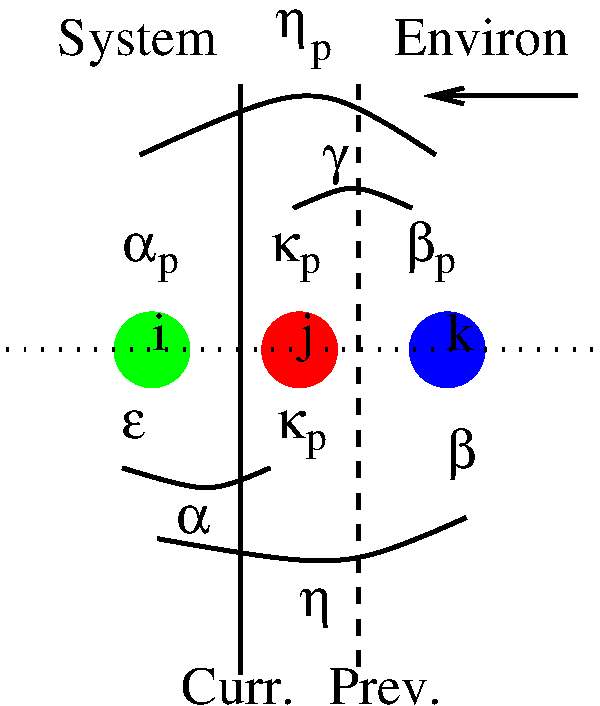
\includegraphics[width=4cm]{wft}}
\caption{TBW.\label{fig:wft}}
\end{figure}
Latin letters label points, Greek letters label states.
The sub-index $p$ indicates the newest DMRG step.
The approximate guess for the new wave-function $\psi^p_{\eta_p}$ is given in terms of the previous 
wave-function $\psi_{\eta}$ by:
\begin{equation}
\psi^p_{\eta_p} = 
W^S_{\alpha,\epsilon}\psi_{\eta}W^E_{\beta,\beta_p}
\delta_{P^{SE}(\eta);\epsilon+\beta n_0}
\delta_{P^S(\alpha);\alpha_{p}+\kappa_{p}n_1}
\delta_{P^S_p(\eta_p);\alpha_p+\gamma_p n_2}
\delta_{P^E_p(\gamma_p);\kappa_p+\beta_p n_3},
\end{equation}
where the system transformation is $W^S$, the environment transformation is $W^E$,
the new system-environment permutation $P^{SE}_p$, the new environment permutation $P^E_p$,
the old system-environment permutation $P^{SE}$, and the new system permutation $P^S$.
A sum should be assumed for all indices except $\eta_p$.
\subsection{SU(2) Reduced Operators}
\subsection{Checkpointing}
\subsection{Distributed Parallelization}
\subsection{Shared-memory Parallelization}

\section{Static Observables}
A quick run with the calculation of static observables can be done like so:
\begin{verbatim}
cd src/
perl configure.pl
(all default answers here)
make
make observe
./dmrg ../TestSuite/input2.inp
./observe ../TestSuite/input2.inp data2.txt
\end{verbatim}
You will see something like this:
\begin{verbatim}
OperatorC:
8 16
0.5 0.426244 -2.84172e-08 ...
0 0.5 -0.252775 1.67222e-07 0.0586682 ...
...
\end{verbatim}
Here we are computing $C_{ij} = \langle c_{i\uparrow}c_{j\uparrow}\rangle$, where $8 16$ are the dimensions of the matrix 
that follow ($C_{ij}$ is not computed for $i>j$).
For example $C_{00}=0.5$, $C_{01}=0.426244$, $C_{12}=-0.252775$. 

The same is done for $N_{ij} = \langle n_{i}n_{j}\rangle$, where $n_i = n_{i\uparrow}+n_{i\downarrow}$, and also for $\langle S_{i}^zS_{j}^z\rangle$

The observer driver (\verb=observe.cpp=) controls what is calculated. Please have a look at it and modify as necessary.

THIS SECTION NEEDS MORE WORK. IN PARTICULAR HOW TO SETUP THE INPUT FILE TO BE ABLE TO PRODUCE DATA FOR THE OBSERVER.


\subsection{Ground State Energy and Error}
\subsection{Static Correlations}
\subsection{Observables Driver}

\section*{LICENSE}
\begin{Verbatim}
Copyright � 2008 , UT-Battelle, LLC
All rights reserved

[DMRG++, Version 2.0.0]
[by G.A., Oak Ridge National Laboratory]

UT Battelle Open Source Software License 11242008

OPEN SOURCE LICENSE

Subject to the conditions of this License, each
contributor to this software hereby grants, free of
charge, to any person obtaining a copy of this software
and associated documentation files (the "Software"), a
perpetual, worldwide, non-exclusive, no-charge,
royalty-free, irrevocable copyright license to use, copy,
modify, merge, publish, distribute, and/or sublicense
copies of the Software.

1. Redistributions of Software must retain the above
copyright and license notices, this list of conditions,
and the following disclaimer.  Changes or modifications
to, or derivative works of, the Software should be noted
with comments and the contributor and organization's
name.

2. Neither the names of UT-Battelle, LLC or the
Department of Energy nor the names of the Software
contributors may be used to endorse or promote products
derived from this software without specific prior written
permission of UT-Battelle.

3. The software and the end-user documentation included
with the redistribution, with or without modification,
must include the following acknowledgment:

"This product includes software produced by UT-Battelle,
LLC under Contract No. DE-AC05-00OR22725  with the
Department of Energy."
 
*********************************************************
DISCLAIMER

THE SOFTWARE IS SUPPLIED BY THE COPYRIGHT HOLDERS AND
CONTRIBUTORS "AS IS" AND ANY EXPRESS OR IMPLIED
WARRANTIES, INCLUDING, BUT NOT LIMITED TO, THE IMPLIED
WARRANTIES OF MERCHANTABILITY AND FITNESS FOR A
PARTICULAR PURPOSE ARE DISCLAIMED. IN NO EVENT SHALL THE
COPYRIGHT OWNER, CONTRIBUTORS, UNITED STATES GOVERNMENT,
OR THE UNITED STATES DEPARTMENT OF ENERGY BE LIABLE FOR
ANY DIRECT, INDIRECT, INCIDENTAL, SPECIAL, EXEMPLARY, OR
CONSEQUENTIAL DAMAGES (INCLUDING, BUT NOT LIMITED TO,
PROCUREMENT OF SUBSTITUTE GOODS OR SERVICES; LOSS OF USE,
DATA, OR PROFITS; OR BUSINESS INTERRUPTION) HOWEVER
CAUSED AND ON ANY THEORY OF LIABILITY, WHETHER IN
CONTRACT, STRICT LIABILITY, OR TORT (INCLUDING NEGLIGENCE
OR OTHERWISE) ARISING IN ANY WAY OUT OF THE USE OF THIS
SOFTWARE, EVEN IF ADVISED OF THE POSSIBILITY OF SUCH
DAMAGE.

NEITHER THE UNITED STATES GOVERNMENT, NOR THE UNITED
STATES DEPARTMENT OF ENERGY, NOR THE COPYRIGHT OWNER, NOR
ANY OF THEIR EMPLOYEES, REPRESENTS THAT THE USE OF ANY
INFORMATION, DATA, APPARATUS, PRODUCT, OR PROCESS
DISCLOSED WOULD NOT INFRINGE PRIVATELY OWNED RIGHTS.

*********************************************************
\end{Verbatim}

\end{document}
